%% The "\appendix" call has already been made in the declaration
%% of the "appendices" environment (see thesis.tex).
\chapter{Double Higgs Boson Production Analysis}
\label{app:doubleHiggs}

\chapterquote{I was an adventurer like you, then I took an arrow in the knee.}
{The town guard, Skyrim, 2011}
% \cite{Skyrim}
%Appendixes (or should that be ``appendices''?) make you look really clever, 'cos
%it's like you had more clever stuff to say than could be fitted into the main
%bit of your thesis. Yeah. So everyone should have at least three of them\dots

Here are extra tables for hadronic decay analysis at \rootS{3} in \Chapter{chap:DoubleHiggs}. \TABLE{tab:doubleHiggs3TeVPreslection} shows the expected number of events, before cuts and after successive cuts: the lepton veto, \eeToHHbbWW/\eeToHHbbbb separation, and valid jet pairing, for the signal and background events at \rootS{3}, assuming an integrated luminosity of 2000\,\uprightMath{fb^{-1}}. \TABLE{tab:doubleHiggs3TeVPreslectionPart2} shows the expected number of events after successive cuts: invariant mass of the two Higgs system > 150\,GeV, and the highest b-jet tag value > 0.7. All cuts include the lepton veto, \eeToHHbbWW/\eeToHHbbbb separation, and valid jet pairing.
%\section{Hadronic decay at \rootS{3} analysis}

\begin{table}[!tbp]\centering
% TODO fix lumi correction for e gamma, gamma e
% TODO change some of sample cross section for  electron-photon interaction with four quarks and a neutrino final state
\small
\begin{tabular}{lrrrr}
\hline \hline
 \multicolumn{1}{L{3.5cm}}{\rootS{3}} &  \multicolumn{1}{R{2cm}}{N}  & \multicolumn{1}{R{2cm}}{Lepton evto} & \multicolumn{1}{R{2cm}}{\bbWW / \bbWW separation} & \multicolumn{1}{R{2cm}}{Valid jet Pairing} \\
\hline
\eeToHH $\to$ \\
\HepProcess{ \Pbottom \APbottom \PWplus \PWminus \Pnue \APnue}, hadronic             &146.0& 80.9\% & 72.8\% & 72.1\%\\
\hline
\eeToHH $\to$ \\
\HepProcess{ \Pbottom \APbottom \Pbottom \APbottom \Pnue \APnue}             &355.0& 83.5\% & 20.5\% & 20.5\% \\
\eeToHH $\to$ other & 675.0 & 40.1\% & 34.3\% & 20.5\% \\
\hline
\eeTo{\qlight \qlight \PHiggs \Pnu \APnu}  & 6120 & 67.7\% & 61.9\% & 61.9\%\\
\eeTo{\Pcharm \APcharm \PHiggs \Pnu \APnu}  & 2300 & 69.1\%& 53.0\%& 48.8\%\\
\eeTo{\Pbottom \APbottom \PHiggs \Pnu \APnu}  & 3560 & 70.1\%& 30.9\%& 30.6\%\\

\eeTo{ \Pquark \Pquark \Pquark \Pquark}   &   1093000& 62.4\% & 44.9\%&34.9\%\\
\eeTo{ \Pquark \Pquark \Pquark \Pquark \Plepton \Plepton}& 338600& 21.4\%& 19.6\%& 13.3\%\\
\eeTo{ \Pquark \Pquark \Pquark \Pquark \Plepton \Pnu}& 213200 & 23.3\%& 19.5\%& 16.3\%\\
\eeTo{ \Pquark \Pquark \Pquark \Pquark \Pnu \APnu} & 143000& 80.7\%& 71.4\%& 50.7\%\\

\eeTo{ \Pquark \Pquark} &  5897800 & 72.9\%& 63.9\%& 55.4\%\\
\eeTo{ \Pquark \Pquark \Plepton \Pnu} &  11121800 & 34.0\%& 24.7\%& 20.5\%\\
\eeTo{ \Pquark \Pquark \Pl \Pl} &  6639200 & 43.1\%& 41.7\%& 37.0\%\\
\eeTo{ \Pquark \Pquark \Pnu \Pnu} & 2635000 &84.6\%& 63.8\%& 53.2\% \\
\hline
\egamma{\Pepm}{\Pphoton}{\BS}{\Pepm \Pquark \Pquark \Pquark \Pquark} & 4007354  & 31.0\%& 28.2\%& 21.1\%\\
%\egamma{\Pem}{\Pphoton}{BS}{\Pem \Pquark \Pquark \Pquark \Pquark} & 2004388.1  & 30.8\%& 28.0\%& 21.0\%\\
%\egamma{\Pep}{\Pphoton}{BS}{\Pep \Pquark \Pquark \Pquark \Pquark} & 2002334.1 & 31.1\%& 28.3\%& 21.1\%\\
\egamma{\Pepm}{\Pphoton}{\EPA}{\Pepm \Pquark \Pquark \Pquark \Pquark} & 1151200& 15.9\%& 14.5\%& 10.9\%\\
%\egamma{\Pem}{\Pphoton}{EPA}{\Pem \Pquark \Pquark \Pquark \Pquark} & 575600.0& 15.9\%& 14.5\%& 10.8\%\\
%\egamma{\Pep}{\Pphoton}{EPA}{\Pep \Pquark \Pquark \Pquark \Pquark}  & 575600.0 & 15.9\% & 14.5\%& 10.9\%\\
\egamma{\Pepm}{\Pphoton}{\BS}{\Pnu \Pquark \Pquark \Pquark \Pquark}& 829184  & 78.3\%& 68.8\%& 53.3\%\\
%\egamma{\Pem}{\Pphoton}{BS}{\Pnu \Pquark \Pquark \Pquark \Pquark}& 414750.0  & 78.2\%& 68.8\%& 53.5\%\\
%\egamma{\Pep}{\Pphoton}{BS}{\APnu \Pquark \Pquark \Pquark \Pquark}& 414434.0 & 78.3\% & 68.7\%& 53.0\%\\
\egamma{\Pepm}{\Pphoton}{\EPA}{\Pnu \Pquark \Pquark \Pquark \Pquark}& 216800  & 39.6\% & 35.0\%& 26.9\%\\
%\egamma{\Pem}{\Pphoton}{EPA}{\Pnu \Pquark \Pquark \Pquark \Pquark}& 108400.0  & 39.6\% & 35.0\%& 26.9\%\\
%\egamma{\Pep}{\Pphoton}{EPA}{\APnu \Pquark \Pquark \Pquark \Pquark}& 108400.0  & 39.5\%& 35.0\%& 26.8\% \\
\egamma{\Pepm}{\Pphoton}{\BS}{\Pquark \Pquark \PHiggs \Pnu} & 185018.0  & 64.0\% &55.4\%& 49.8\% \\
%\egamma{\Pem}{\Pphoton}{BS}{\Pquark \Pquark \PHiggs \Pnu} & 92588.0  & 64.1\% &55.4\%& 49.8\% \\
%\egamma{\Pep}{\Pphoton}{BS}{\Pquark \Pquark \PHiggs \Pnu} & 92430.0 & 63.9\% & 55.4\% & 49.8\% \\
\egamma{\Pepm}{\Pphoton}{\EPA}{\Pquark \Pquark \PHiggs \Pnu} & 46800 & 32.9\% &28.8\% & 25.9\% \\
%\egamma{\Pem}{\Pphoton}{EPA}{\Pquark \Pquark \PHiggs \Pnu} & 23400.0 & 33.2\% &29.0\% & 26.1\% \\
%\egamma{\Pep}{\Pphoton}{EPA}{\Pquark \Pquark \PHiggs \Pnu} & 23400.0   & 32.6\% & 28.6\% & 25.7\% \\
\hline
\gammagamma{\Pphoton}{\BS}{\Pphoton}{\BS}{ \Pquark \Pquark \Pquark \Pquark}& 18009414  & 71.6\%& 65.5\%& 49.4\%\\
\gammagamma{\Pphoton}{\BS}{\Pphoton}{\EPA}{ \Pquark \Pquark \Pquark \Pquark}& 3824548  &44.3\%& 40.6\%& 30.6\%\\
\gammagamma{\Pphoton}{\EPA}{\Pphoton}{\BS}{ \Pquark \Pquark \Pquark \Pquark}& 3828498 & 44.3\%& 40.7\%& 30.7\%\\
\gammagamma{\Pphoton}{\EPA}{\Pphoton}{\EPA}{ \Pquark \Pquark \Pquark \Pquark}& 805400 & 29.0\% & 26.7\% & 20.1\%\\
\hline \hline
\end{tabular}

\caption
{The table shows the expected number of events, before cuts and after successive cuts: the lepton veto, \eeToHHbbWW/\eeToHHbbbb separation, and valid jet pairing, for the signal and background events at \rootS{3}, assuming an integrated luminosity of 2000\,\uprightMath{fb^{-1}}. \Pquark can be \Pup, \Pdown, \Pstrange, \Pbottom or \Ptop. Unless specified, \Pquark, \Plepton and \Pnu represent either particles or the corresponding anti-particles.}
\label{tab:doubleHiggs3TeVPreslection}
\end{table}



\begin{table}[!tbp]\centering

\begin{tabular}{lrr}
\hline \hline
 \multicolumn{1}{L{0.3\textwidth}}{Process} &  \multicolumn{1}{R{0.3\textwidth}}{$m_{\HH}$>150GeV}  & \multicolumn{1}{R{0.3\textwidth}}{$B_1$>0.7} \\
\hline
\eeToHH $\to$ \\
\HepProcess{ \Pbottom \APbottom \PWplus \PWminus \Pnue \APnue}, hadronic             & 71.7\% & 61.8\%\\
\hline
\eeToHH $\to$ \\
\HepProcess{ \Pbottom \APbottom \Pbottom \APbottom \Pnue \APnue}             & 20.2\% & 18.8\% \\
\eeToHH $\to$ other & 30.2\% & 20.0\% \\
\hline
\eeTo{\qlight \qlight \PHiggs \Pnu \APnu}   & 53.1\% & 36.0\%\\
\eeTo{\Pcharm \APcharm \PHiggs \Pnu \APnu} & 43.8\%& 26.3\%\\
\eeTo{\Pbottom \APbottom \PHiggs \Pnu \APnu} & 29.6\%& 25.9\%\\

\eeTo{ \Pquark \Pquark \Pquark \Pquark}   & 26.5\%& 1.7\%\\
\eeTo{ \Pquark \Pquark \Pquark \Pquark \Plepton \Plepton} & 12.8\%& 0.7\%\\
\eeTo{ \Pquark \Pquark \Pquark \Pquark \Plepton \Pnu} & 16.0\%& 7.9\%\\
\eeTo{ \Pquark \Pquark \Pquark \Pquark \Pnu \APnu} &49.7\%& 9.0\%\\

\eeTo{ \Pquark \Pquark} & 8.3\%& 1.4\%\\
\eeTo{ \Pquark \Pquark \Plepton \Pnu} & 6.0\%& 0.1\%\\
\eeTo{ \Pquark \Pquark \Pl \Pl} & 1.9\%& 0.4\%\\
\eeTo{ \Pquark \Pquark \Pnu \Pnu} & 16.6\%& 3.1\% \\
\hline
\egamma{\Pepm}{\Pphoton}{\BS}{\Pepm \Pquark \Pquark \Pquark \Pquark}& 19.4\%& 0.7\%\\
%\egamma{\Pem}{\Pphoton}{BS}{\Pem \Pquark \Pquark \Pquark \Pquark}& 19.3\%& 0.7\%\\
%\egamma{\Pep}{\Pphoton}{BS}{\Pep \Pquark \Pquark \Pquark \Pquark} & 19.4%& 0.7\%\\
\egamma{\Pepm}{\Pphoton}{\EPA}{\Pepm \Pquark \Pquark \Pquark \Pquark} & 9.9\%& 0.4\%\\
%\egamma{\Pem}{\Pphoton}{EPA}{\Pem \Pquark \Pquark \Pquark \Pquark} & 09.9\%& 0.4%\\
%\egamma{\Pep}{\Pphoton}{EPA}{\Pep \Pquark \Pquark \Pquark \Pquark}   & 9.9\%& 0.4\%\\
\egamma{\Pepm}{\Pphoton}{\BS}{\Pnu \Pquark \Pquark \Pquark \Pquark} & 51.3\%& 16.4\%\\
%\egamma{\Pem}{\Pphoton}{BS}{\Pnu \Pquark \Pquark \Pquark \Pquark} & 51.5\%& 16.8\%\\
%\egamma{\Pep}{\Pphoton}{BS}{\APnu \Pquark \Pquark \Pquark \Pquark} & 51.1\%& 15.9\%\\
\egamma{\Pepm}{\Pphoton}{\EPA}{\Pnu \Pquark \Pquark \Pquark \Pquark} & 26.0\%& 7.7\%\\
%\egamma{\Pem}{\Pphoton}{EPA}{\Pnu \Pquark \Pquark \Pquark \Pquark} & 26.0\%& 7.9\%\\
%\egamma{\Pep}{\Pphoton}{EPA}{\APnu \Pquark \Pquark \Pquark \Pquark}& 25.9\%& 7.5\% \\
\egamma{\Pepm}{\Pphoton}{\BS}{\Pquark \Pquark \PHiggs \Pnu} &47.9\%& 30.3\% \\
%\egamma{\Pem}{\Pphoton}{BS}{\Pquark \Pquark \PHiggs \Pnu} &47.9\%& 30.2\% \\
%\egamma{\Pep}{\Pphoton}{BS}{\Pquark \Pquark \PHiggs \Pnu} & 47.9\% & 30.3\% \\
\egamma{\Pem}{\Pphoton}{\EPA}{\Pquark \Pquark \PHiggs \Pnu} & 25.0\% & 15.8\% \\
%\egamma{\Pem}{\Pphoton}{EPA}{\Pquark \Pquark \PHiggs \Pnu} & 25.2\% & 16.0\% \\
%\egamma{\Pep}{\Pphoton}{EPA}{\Pquark \Pquark \PHiggs \Pnu} & 24.8\% & 15.6\% \\
\hline
\gammagamma{\Pphoton}{\BS}{\Pphoton}{\BS}{ \Pquark \Pquark \Pquark \Pquark}& 44.5\%& 1.7\%\\
\gammagamma{\Pphoton}{\BS}{\Pphoton}{\EPA}{ \Pquark \Pquark \Pquark \Pquark}& 27.4\%& 1.0\%\\
\gammagamma{\Pphoton}{\EPA}{\Pphoton}{\BS}{ \Pquark \Pquark \Pquark \Pquark}& 27.5\%& 1.0\%\\
\gammagamma{\Pphoton}{\EPA}{\Pphoton}{\EPA}{ \Pquark \Pquark \Pquark \Pquark} & 18.0\% & 0.7\%\\
\hline \hline
\end{tabular}
\caption
{The table shows the expected number of events after successive cuts: invariant mass of the two Higgs system > 150\,GeV, and the highest b-jet tag value > 0.7. All cuts include the lepton veto, \eeToHHbbWW/\eeToHHbbbb separation, and valid jet pairing. \HiggsTableHigh
}
\label{tab:doubleHiggs3TeVPreslectionPart2}
\end{table}


 \begin{figure}[!htbp]
  \begin{subfigure}[b]{0.45\textwidth}
    \includegraphics[width=\textwidth]{{doubleHiggs/1400var/nR0_7_6jet_btag2_W_Onshell_M_TMVA20161208R0_7_qq_btag2_prepare_testNew2}.pdf}
    \caption{}
  \end{subfigure}
    \begin{subfigure}[b]{0.45\textwidth}
    \includegraphics[width=\textwidth]{{doubleHiggs/1400var/nR0_7_6jet_btag2_Higgs_all_M_TMVA20161208R0_7_qq_btag2_prepare_testNew2}.pdf}
    \caption{}
  \end{subfigure}
    \begin{subfigure}[b]{0.45\textwidth}
    \includegraphics[width=\textwidth]{{doubleHiggs/1400var/nR0_7_6jet_btag2_W_Offshell_E_TMVA20161208R0_7_qq_btag2_prepare_testNew2}.pdf}
    \caption{}
  \end{subfigure}
    \begin{subfigure}[b]{0.45\textwidth}
    \includegraphics[width=\textwidth]{{doubleHiggs/1400var/nR0_7_6jet_btag2_Higgs1_Pt_TMVA20161208R0_7_qq_btag2_prepare_testNew2}.pdf}
    \caption{}
  \end{subfigure}
    \begin{subfigure}[b]{0.45\textwidth}
    \includegraphics[width=\textwidth]{{doubleHiggs/1400var/nR0_7_6jet_btag2_Higgs2_Pt_TMVA20161208R0_7_qq_btag2_prepare_testNew2}.pdf}
    \caption{}
  \end{subfigure}
    \begin{subfigure}[b]{0.45\textwidth}
    \includegraphics[width=\textwidth]{{doubleHiggs/1400var/nR0_7_6jet_btag2_Higgs_all_Pt_TMVA20161208R0_7_qq_btag2_prepare_testNew2}.pdf}
    \caption{}
  \end{subfigure}
\caption
   {Distributions of: a)  the invariant mass of  \PW ($m_{\PW}$); b) the invariant mass of the double Higgs system ($m_{\HH}$); c) the energy of the off-mass-shell \PW ($E_{\W*}$); d) the transverse momentum of \Hbb ($\pT_{\Hbb}$); e) the transverse momentum of \HWW ($\pT_{\HWW}$); and f) the transverse momentum of the double Higgs system ($\pT_{\HH}$). All plots assume an integrated luminosity of  1500\,\uprightMath{fb^{-1}} at \rootS{1.4} after all pre-selection cuts applied before the MVA event selection.}
   \label{fig:doubleHiggs1.4var2}
\end{figure}

 \begin{figure}[!htbp]
  \begin{subfigure}[b]{0.45\textwidth}
    \includegraphics[width=\textwidth]{{doubleHiggs/1400var/nR0_7_6jet_btag2_Recoil_pseudorapidity_TMVA20161208R0_7_qq_btag2_prepare_testNew2}.pdf}
    \caption{}
  \end{subfigure}
    \begin{subfigure}[b]{0.45\textwidth}
    \includegraphics[width=\textwidth]{{doubleHiggs/1400var/nR0_7_6jet_btag2_W_Onshell_acolinearity_TMVA20161208R0_7_qq_btag2_prepare_testNew2}.pdf}
    \caption{}
  \end{subfigure}
    \begin{subfigure}[b]{0.45\textwidth}
    \includegraphics[width=\textwidth]{{doubleHiggs/1400var/nR0_7_6jet_btag2_Higgs_all_M_TMVA20161208R0_7_qq_btag2_prepare_testNew2}.pdf}
    \caption{}
  \end{subfigure}
    \begin{subfigure}[b]{0.45\textwidth}
    \includegraphics[width=\textwidth]{{doubleHiggs/1400var/nR0_7_6jet_btag2_Higgs2_spin_TMVA20161208R0_7_qq_btag2_prepare_testNew2}.pdf}
    \caption{}
  \end{subfigure}
    \begin{subfigure}[b]{0.45\textwidth}
    \includegraphics[width=\textwidth]{{doubleHiggs/1400var/nR0_7_6jet_btag2_W_Onshell_spin_TMVA20161208R0_7_qq_btag2_prepare_testNew2}.pdf}
    \caption{}
  \end{subfigure}
    \begin{subfigure}[b]{0.45\textwidth}
    \includegraphics[width=\textwidth]{{doubleHiggs/1400var/nR0_7_6jet_btag2_W_Offshell_spin_TMVA20161208R0_7_qq_btag2_prepare_testNew2}.pdf}
    \caption{}
  \end{subfigure}
\caption
   {Distributions of: a)   the pseudorapidity of the missing momenta ($\eta_{mis}$); b) the  acollinearity of the two jets associated with \HWW ($\acolinearity{\HWW}$); c) the  acollinearity of the two Higgs bosons ($\acolinearity{\HH}$); d) the angle between the  two \PW{s} associated with \HWW in the \HWW decay rest frame and the direction of  to the direction of \Hbb  ($\cosStar{\HWW}$); e) the angle between the two jets associated with \PW in the \PW decay rest frame and the direction of  to the direction of \PW ($\cosStar{\PW}$); and f) the angle between the two jets associated with \W* in the \W* decay rest frame and the direction of  to the direction of  \W*  ($\cosStar{\W*}$).  All plots assume an integrated luminosity of  1500\,\uprightMath{fb^{-1}} at \rootS{1.4} after all pre-selection cuts applied before the MVA event selection.}
   \label{fig:doubleHiggs1.4var3}
\end{figure}

 \begin{figure}[!htbp]
  \begin{subfigure}[b]{0.45\textwidth}
    \includegraphics[width=\textwidth]{{doubleHiggs/1400var/nR0_7_6jet_btag2_Higgs_all_spin_TMVA20161208R0_7_qq_btag2_prepare_testNew2}.pdf}
    \caption{}
  \end{subfigure}
    \begin{subfigure}[b]{0.45\textwidth}
    \includegraphics[width=\textwidth]{{doubleHiggs/1400var/sphericity_TMVA20161208R0_7_qq_btag2_prepare_testNew2}.pdf}
    \caption{}
  \end{subfigure}
    \begin{subfigure}[b]{0.45\textwidth}
    \includegraphics[width=\textwidth]{{doubleHiggs/1400var/nR0_7_6jet_btag2_minusLogY23_TMVA20161208R0_7_qq_btag2_prepare_testNew2}.pdf}
    \caption{}
  \end{subfigure}
    \begin{subfigure}[b]{0.45\textwidth}
    \includegraphics[width=\textwidth]{{doubleHiggs/1400var/nR0_7_6jet_btag2_minusLogY34_TMVA20161208R0_7_qq_btag2_prepare_testNew2}.pdf}
    \caption{}
  \end{subfigure}
    \begin{subfigure}[b]{0.45\textwidth}
    \includegraphics[width=\textwidth]{{doubleHiggs/1400var/nR0_7_6jet_btag2_minusLogY45_TMVA20161208R0_7_qq_btag2_prepare_testNew2}.pdf}
    \caption{}
  \end{subfigure}
    \begin{subfigure}[b]{0.45\textwidth}
    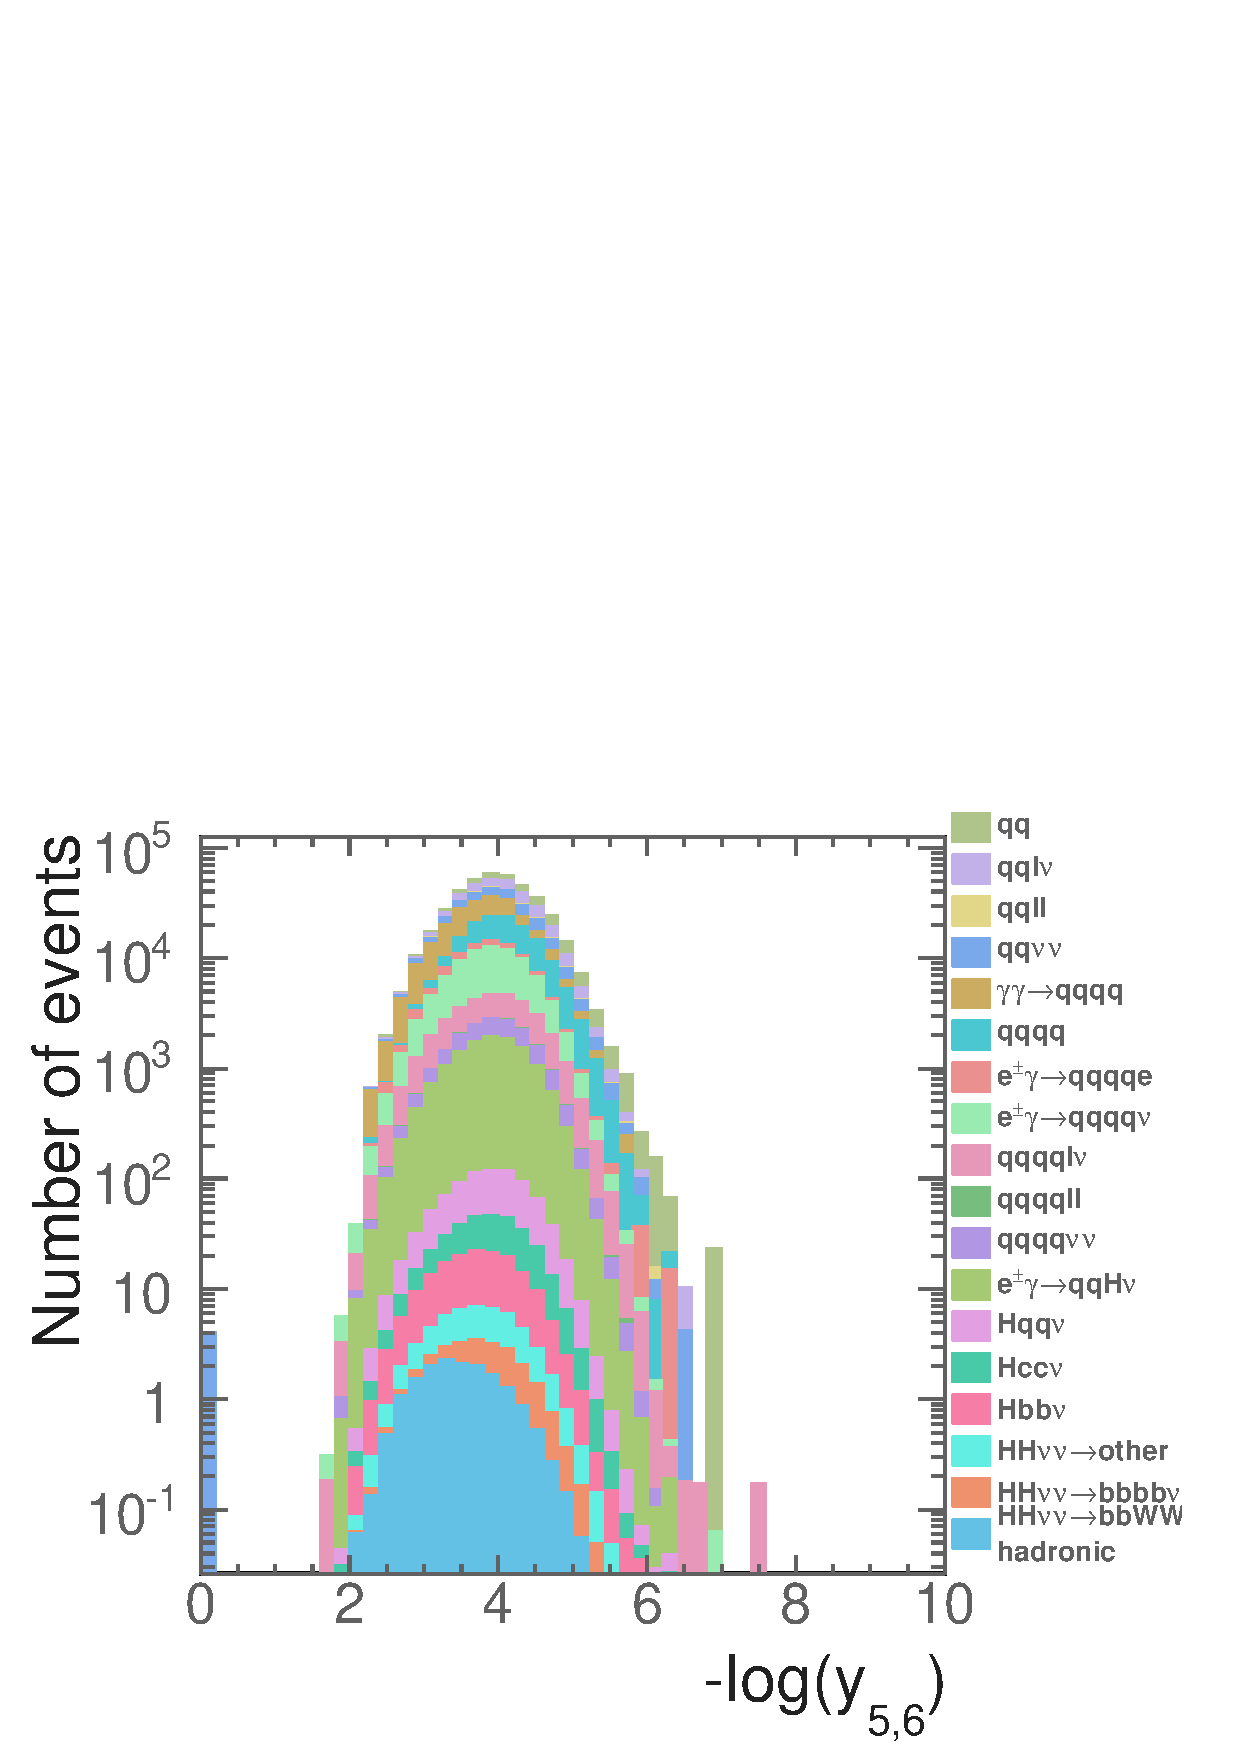
\includegraphics[width=\textwidth]{{doubleHiggs/1400var/nR0_7_6jet_btag2_minusLogY56_TMVA20161208R0_7_qq_btag2_prepare_testNew2}.pdf}
    \caption{}
  \end{subfigure}
\caption
   {Distributions of: a)   the angle between the two Higgs bosons in two Higgs bosons decay rest frame and the direction of  to the direction of  the two Higgs boson  ($\cosStar{\HH}$); b)  the absolute value of the sphericity ($\abs{\sphericity}$); c) the negative logarithm of \y{23} ($-\ln(\y{23})$); d) the negative logarithm of \y{34} ($-\ln(\y{34})$); e) the negative logarithm of \y{45} ($-\ln(\y{45})$); and f) the negative logarithm of \y{56} ($-\ln(\y{56})$).    All plots assume an integrated luminosity of  1500\,\uprightMath{fb^{-1}} at \rootS{1.4} after all pre-selection cuts applied before the MVA event selection.}
   \label{fig:doubleHiggs1.4var4}
\end{figure}


 \begin{figure}[!htbp]
  \begin{subfigure}[b]{0.45\textwidth}
    \includegraphics[width=\textwidth]{{doubleHiggs/1400var/nR0_7_6jet_btag2_Higgs1_bTag1_TMVA20161208R0_7_qq_btag2_prepare_testNew2}.pdf}
    \caption{}
  \end{subfigure}
    \begin{subfigure}[b]{0.45\textwidth}
    \includegraphics[width=\textwidth]{{doubleHiggs/1400var/nR0_7_6jet_btag2_Higgs1_bTag2_TMVA20161208R0_7_qq_btag2_prepare_testNew2}.pdf}
    \caption{}
  \end{subfigure}
    \begin{subfigure}[b]{0.45\textwidth}
    \includegraphics[width=\textwidth]{{doubleHiggs/1400var/nR0_7_6jet_btag2_W_Onshell_bTag1_TMVA20161208R0_7_qq_btag2_prepare_testNew2}.pdf}
    \caption{}
  \end{subfigure}
    \begin{subfigure}[b]{0.45\textwidth}
    \includegraphics[width=\textwidth]{{doubleHiggs/1400var/nR0_7_6jet_btag2_W_Offshell_bTag1_TMVA20161208R0_7_qq_btag2_prepare_testNew2}.pdf}
    \caption{}
  \end{subfigure}
    \begin{subfigure}[b]{0.45\textwidth}
    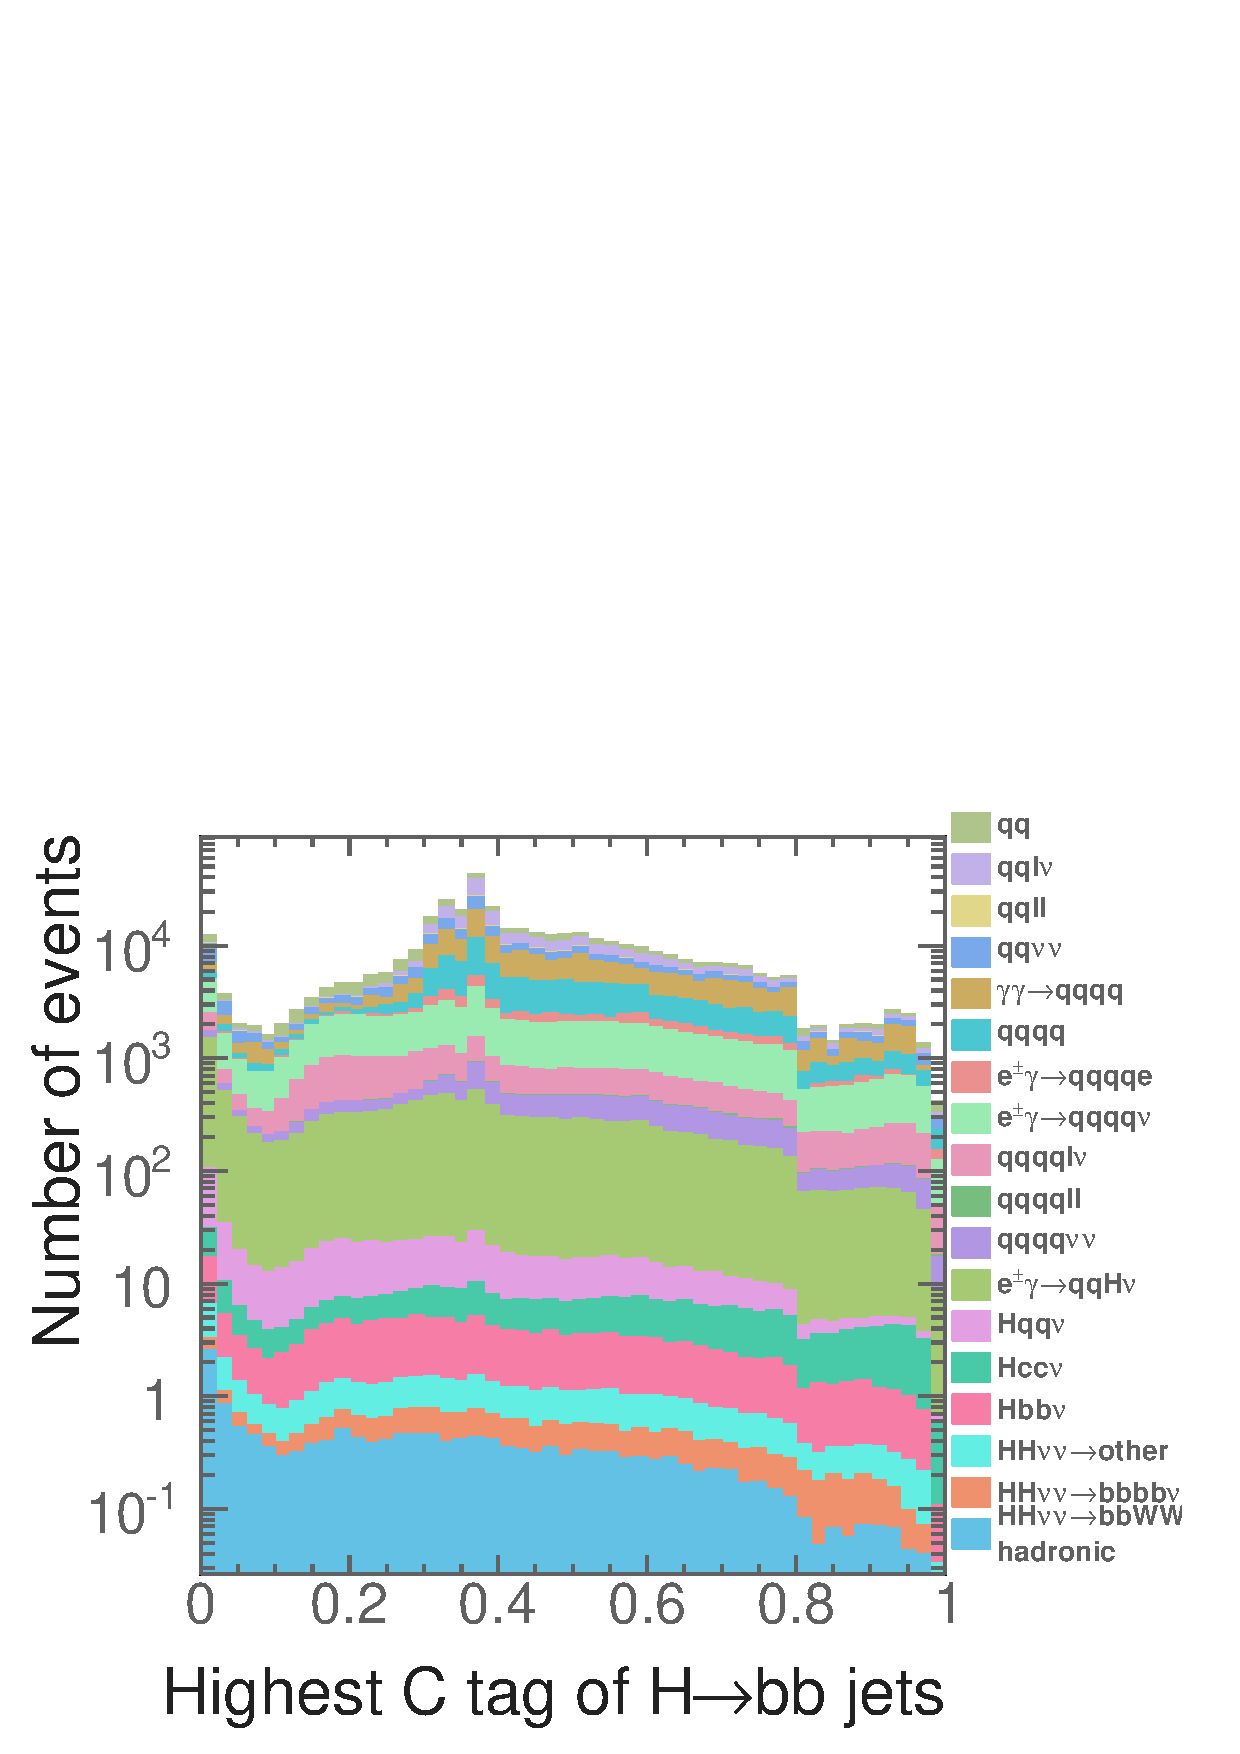
\includegraphics[width=\textwidth]{{doubleHiggs/1400var/nR0_7_6jet_btag2_Higgs1_cTag1_TMVA20161208R0_7_qq_btag2_prepare_testNew2}.pdf}
    \caption{}
  \end{subfigure}
    \begin{subfigure}[b]{0.45\textwidth}
    \includegraphics[width=\textwidth]{{doubleHiggs/1400var/nR0_7_6jet_btag2_W_Onshell_cTag1_TMVA20161208R0_7_qq_btag2_prepare_testNew2}.pdf}
    \caption{}
  \end{subfigure}
\caption
   {Distributions of: a)   the highest b-jet tag value of the two jets associated with \Hbb ($\btagFull{1}{\Hbb}$); b) the lowest b-jet tag value of the two jets associated with \Hbb ($\btagFull{2}{\Hbb}$); c) the highest b-jet tag value of the two jets associated with \PW ($\btagFull{1}{\PW}$); d) the highest b-jet tag value of the two jets associated with \W* ($\btagFull{1}{\W*}$); e) the highest c-jet tag value of the two jets associated with \Hbb ($\ctagFull{1}{\Hbb}$); and f) the highest c-jet tag value of the two jets associated with \PW ($\ctagFull{1}{\PW}$).  All plots assume an integrated luminosity of  1500\,\uprightMath{fb^{-1}} at \rootS{1.4} after all pre-selection cuts applied before the MVA event selection.}
   \label{fig:doubleHiggs1.4var5}
\end{figure}

 \begin{figure}[!htbp]
    \begin{subfigure}[b]{0.45\textwidth}
    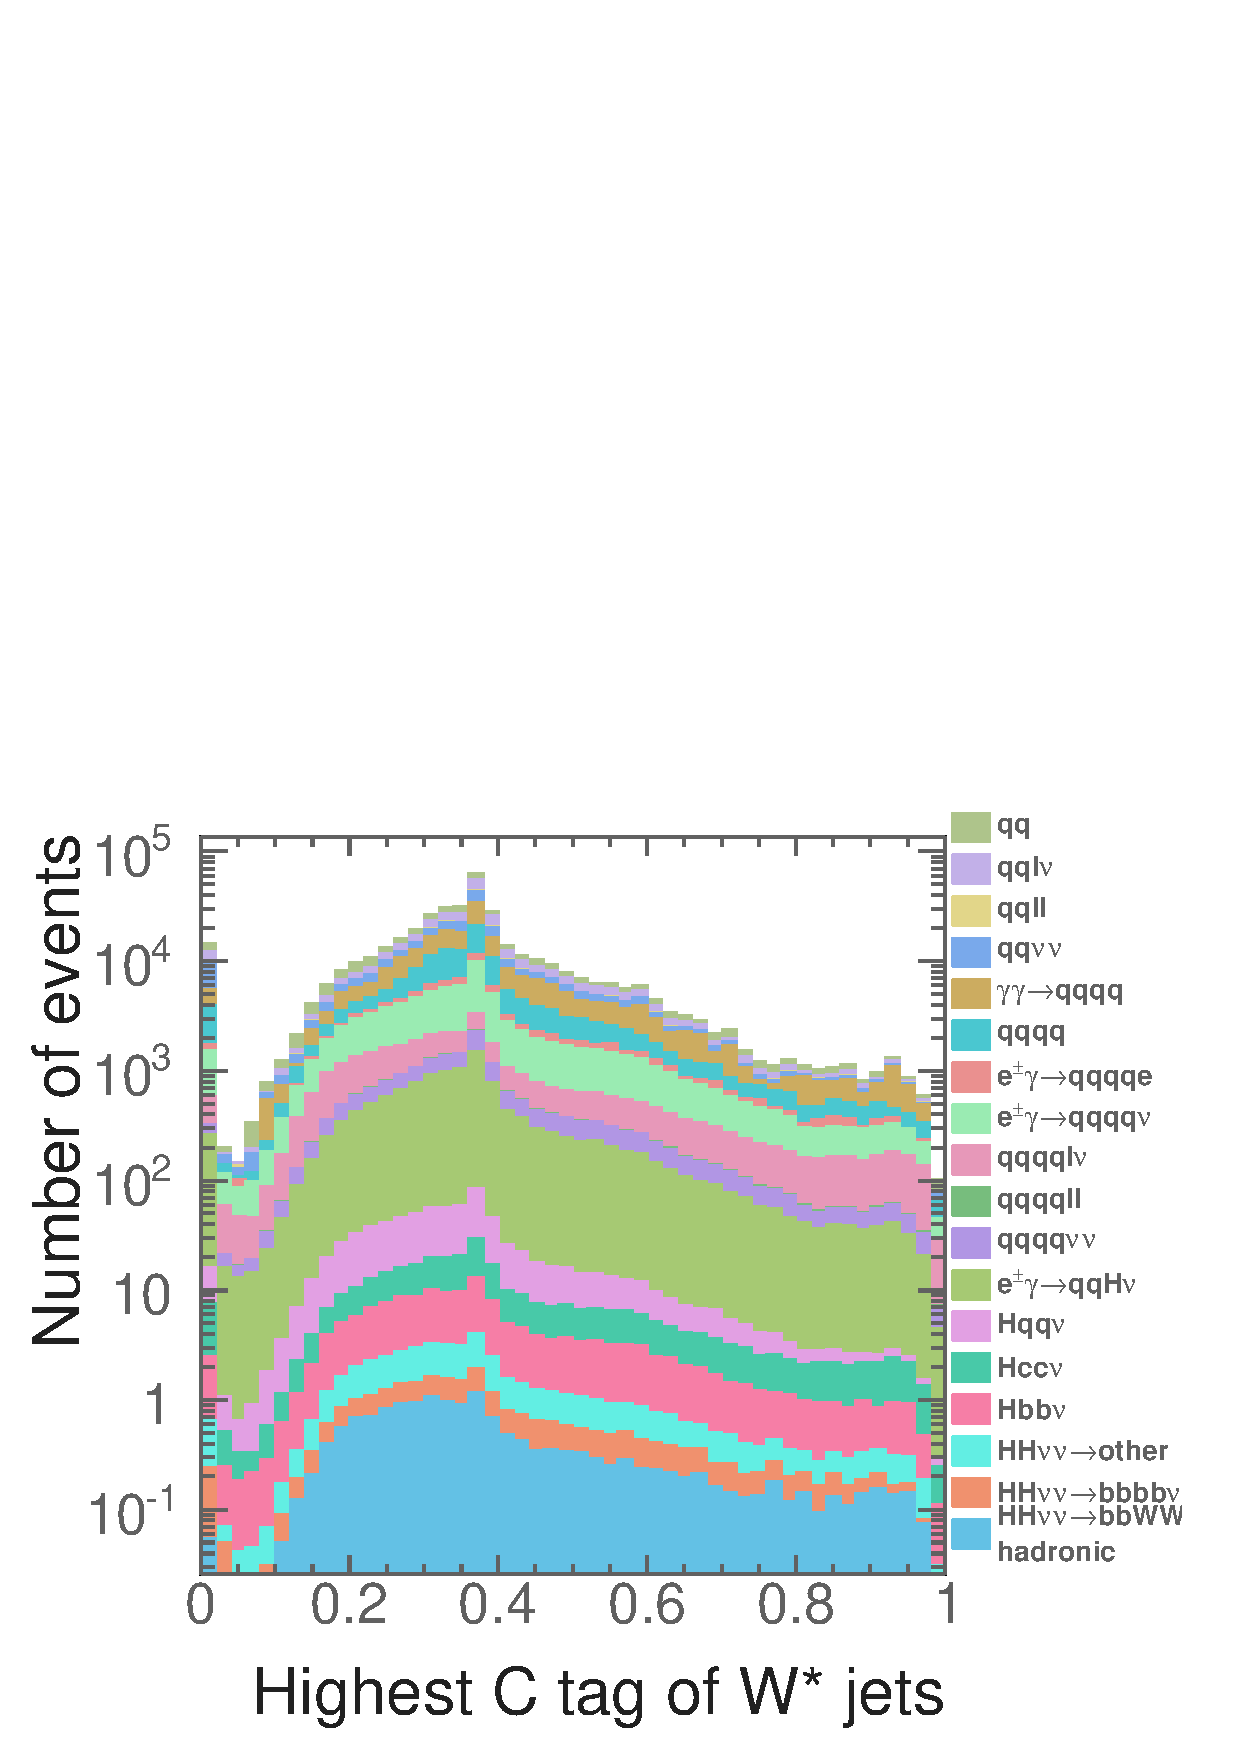
\includegraphics[width=\textwidth]{{doubleHiggs/1400var/nR0_7_6jet_btag2_W_Offshell_cTag1_TMVA20161208R0_7_qq_btag2_prepare_testNew2}.pdf}
    \caption{}
  \end{subfigure}
  \begin{subfigure}[b]{0.45\textwidth}
    \includegraphics[width=\textwidth]{{doubleHiggs/1400var/nR0_7_6jet_btag2_Higgs1_nPfo_TMVA20161208R0_7_qq_btag2_prepare_testNew2}.pdf}
    \caption{}
  \end{subfigure}
    \begin{subfigure}[b]{0.45\textwidth}
    \includegraphics[width=\textwidth]{{doubleHiggs/1400var/nR0_7_6jet_btag2_W_Onshell_nPfo_TMVA20161208R0_7_qq_btag2_prepare_testNew2}.pdf}
    \caption{}
  \end{subfigure}
    \begin{subfigure}[b]{0.45\textwidth}
    \includegraphics[width=\textwidth]{{doubleHiggs/1400var/nR0_7_6jet_btag2_W_Offshell_nPfo_TMVA20161208R0_7_qq_btag2_prepare_testNew2}.pdf}
    \caption{}
  \end{subfigure}
\caption
   {Distributions of: a) the highest c-jet tag value of the two jets associated with \W* ($\ctagFull{1}{\W*}$); b) the number of particles associated with \Hbb (\npfo{\Hbb}); c) the number of particles associated with \PW (\npfo{\PW}); and d) the number of particles associated with \W* (\npfo{\W*}).  All plots assume an integrated luminosity of  1500\,\uprightMath{fb^{-1}} at \rootS{1.4} after all pre-selection cuts applied before the MVA event selection.}
   \label{fig:doubleHiggs1.4var6}
\end{figure}

%% Big appendixes should be split off into separate files, just like chapters
%\input{app-myreallybigappendix}
